\documentclass{beamer}
 
\usepackage[utf8]{inputenc}
\usepackage{svg}
\usepackage{tikz}
\usepackage{amsmath}
\usepackage[customcolors]{hf-tikz}


\definecolor{amber}{rgb}{1.0, 0.75, 0.0}
\definecolor{generator}{rgb}{0.67, 0.9, 0.93}
\definecolor{discriminator}{rgb}{0.89, 0.44, 0.48}

\usetheme{metropolis}
 
 
\title[GAN] %optional
{GAN - Theory and Applications}
  
\author % (optional, for multiple authors)
{Michele de Simoni  \and  \\ Paolo Galeone \and \\ Emanuele Ghelfi \and \\ Federico di Mattia}
 

 
\titlegraphic{
	 \begin{picture}(0,0)
	\put(100,25){\makebox(0,0)[rt]{
	
\includegraphics[height=1.5cm]{zuru-logo.png}}}
\end{picture}
}
 
 
 
\begin{document}
 
{
  \usebackgroundtemplate{
  	\tikz[overlay,remember picture] \node[opacity=0.2, at=(current page.center)] {
  		\includesvg[width=0.5\textwidth]{pycon_x_logo.svg}};}
  \begin{frame}
    \titlepage
  \end{frame}
}

 
\begin{frame}
\frametitle{Generative Adversarial Networks}

\setbeamercolor{block body}{bg=amber!20!white}
\begin{block}{}
	{\large ``Adversarial Training (also called GAN for Generative Adversarial Networks) is the most interesting idea in the last 10 years of ML.''}
	\vskip5mm
	\hspace*\fill{\small--- Yann LeCun}
\end{block}

\end{frame}

\begin{frame}
\frametitle{Generative Adversarial Networks}
	Two components, the \textbf{generator} and the \textbf{discriminator}:
	\begin{itemize}
		\item The \textbf{generator} G, aim is to capture the data distribution.
		\item The \textbf{discriminator} D, estimates the probability that a sample came from the training data rather than from G.
	\end{itemize}

\begin{figure}
	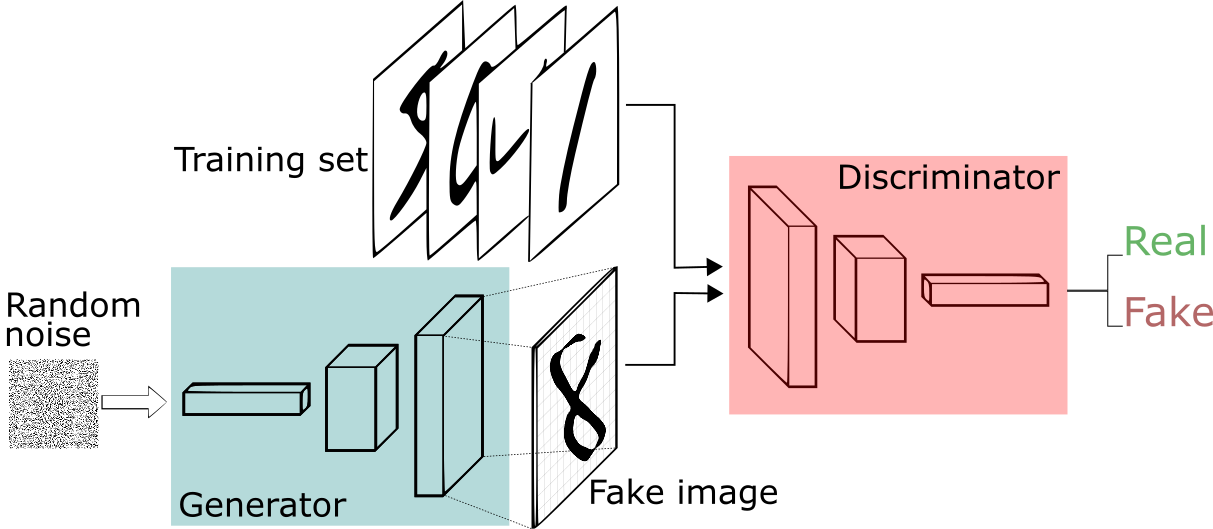
\includegraphics[width=\textwidth]{GANs.png}
	\caption{Credits: Reference  }
\end{figure}

\end{frame}

\begin{frame}
\frametitle{Generative Adversarial Networks}
Generator and Discriminator compete against each other, playing the following \textbf{zero sum min-max game} with value function $V_{GAN}(D,G)$:
\only<1>{
\begin{equation}
 \min_G \max_D V_{GAN}(D,G) = \underset{x \sim p_{data}(x)}{\mathbb{E}} [\log D(x)]  +\underset{z \sim p_z(z)}{\mathbb{E}}[\log(1 - D(G(z)))]
\end{equation}
}

\only<2>{
	\begin{equation}
	\min_G \max_D V_{GAN}(D,G) =\underbrace{\underset{x \sim p_{data}(x)}{\mathbb{E}} [\log D(x)]}_{\text{real samples}}  +\underset{z \sim p_z(z)}{\mathbb{E}}[\log(1 - D(G(z)))]
	\end{equation}
}

\only<3>{
	\begin{equation}
	\min_G \max_D V_{GAN}(D,G) =\underbrace{\underset{x \sim p_{data}(x)}{\mathbb{E}} [\log D(x)]}_{\text{real samples}}  +\underbrace{\underset{z \sim p_z(z)}{\mathbb{E}}[\log(1 - D(G(z)))]}_{\text{generated samples}}
	\end{equation}
}

\end{frame}

\begin{frame}
\frametitle{GANs - Discriminator}
Intuitive explanation:
\begin{itemize}
	\item \textbf{Discriminator} needs to:
	\begin{itemize}
		\hfsetfillcolor{discriminator!50}
		\hfsetbordercolor{discriminator}
		\item Correctly classify real data: \\  \begin{equation} \tikzmarkin{a}(0.2,-0.5)(-0.2,0.65) \max_D \underset{x \sim p_{data}(x)}{\mathbb{E}} [\log D(x)].\tikzmarkend{a}
		\end{equation}
		\item Correctly classify wrong data: \\  \begin{equation}
		\hfsetfillcolor{discriminator!50}
		\hfsetbordercolor{discriminator} \tikzmarkin{b}(0.2,-0.5)(-0.2,0.65) \max_D  \underset{z \sim p_z(z)}{\mathbb{E}}[\log(1 - D(G(z)))].\tikzmarkend{b} \end{equation}
	\end{itemize}
\end{itemize}
\end{frame}

\begin{frame}
\frametitle{GANs - Generator}
Intuitive explanation:
\begin{itemize}
	\item \textbf{Generator} needs to \textbf{fool} the discriminator:
	\begin{itemize}
		\hfsetfillcolor{generator!50}
		\hfsetbordercolor{generator}
		\onslide<1->{
		\item Generate samples similar to the real one: \begin{equation} \tikzmarkin{c}(0.2,-0.5)(-0.2,0.65) \min_G  \underset{z \sim p_z(z)}{\mathbb{E}}[\log(1 - D(G(z)))].\tikzmarkend{c}
		\end{equation}
	}
		\onslide<2->{
			\item Saturates easily \cite{gan}.
			\item Change loss for generator:
			\begin{equation} \tikzmarkin{e}(0.2,-0.5)(-0.2,0.65) \max_G  \underset{z \sim p_z(z)}{\mathbb{E}}[\log( D(G(z)))].\tikzmarkend{e}
			\end{equation}
		}
	\end{itemize}
\end{itemize}
\end{frame}

\begin{frame}
	\frametitle{GANs - Models definition}
	\begin{itemize}
		\item Both D and G can be parametrized functions (Neural Networks).
		\item Different architectures to reach different aims.
		\begin{itemize}
			\only<1>{\item Tuple of numbers? \begin{figure}
					\centering
					\includesvg[width=0.8\textwidth]{nn.svg}
			\end{figure}}
		\only<2>{\item Text or sequences? \begin{figure}
				\hspace{-1cm}
				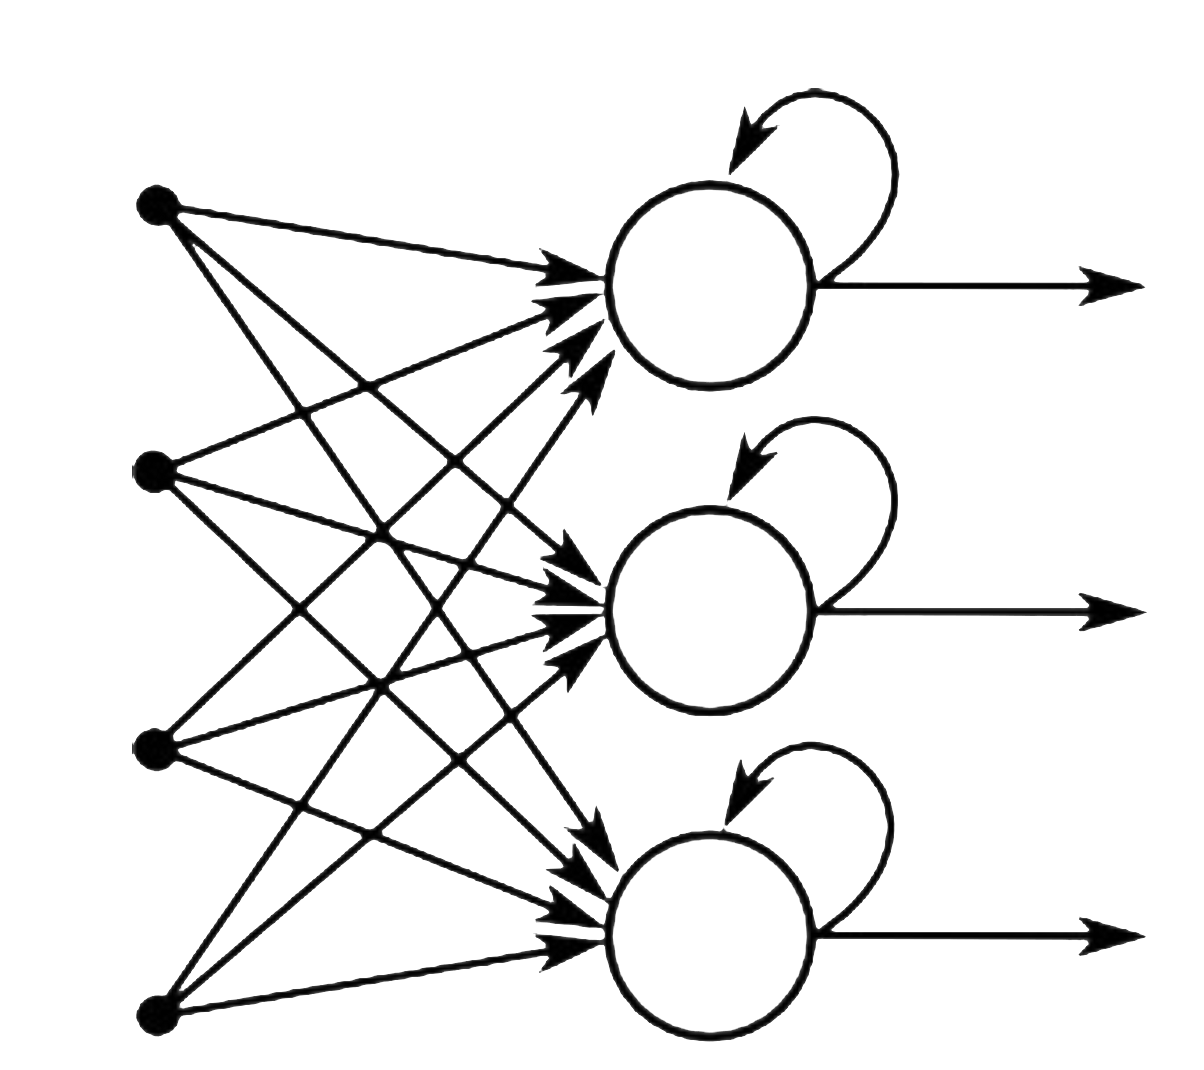
\includegraphics[width=0.5\textwidth]{recurrent.png}
		\end{figure}}
		\only<3>{\item Images? \begin{figure}
			\hspace{-1cm}
			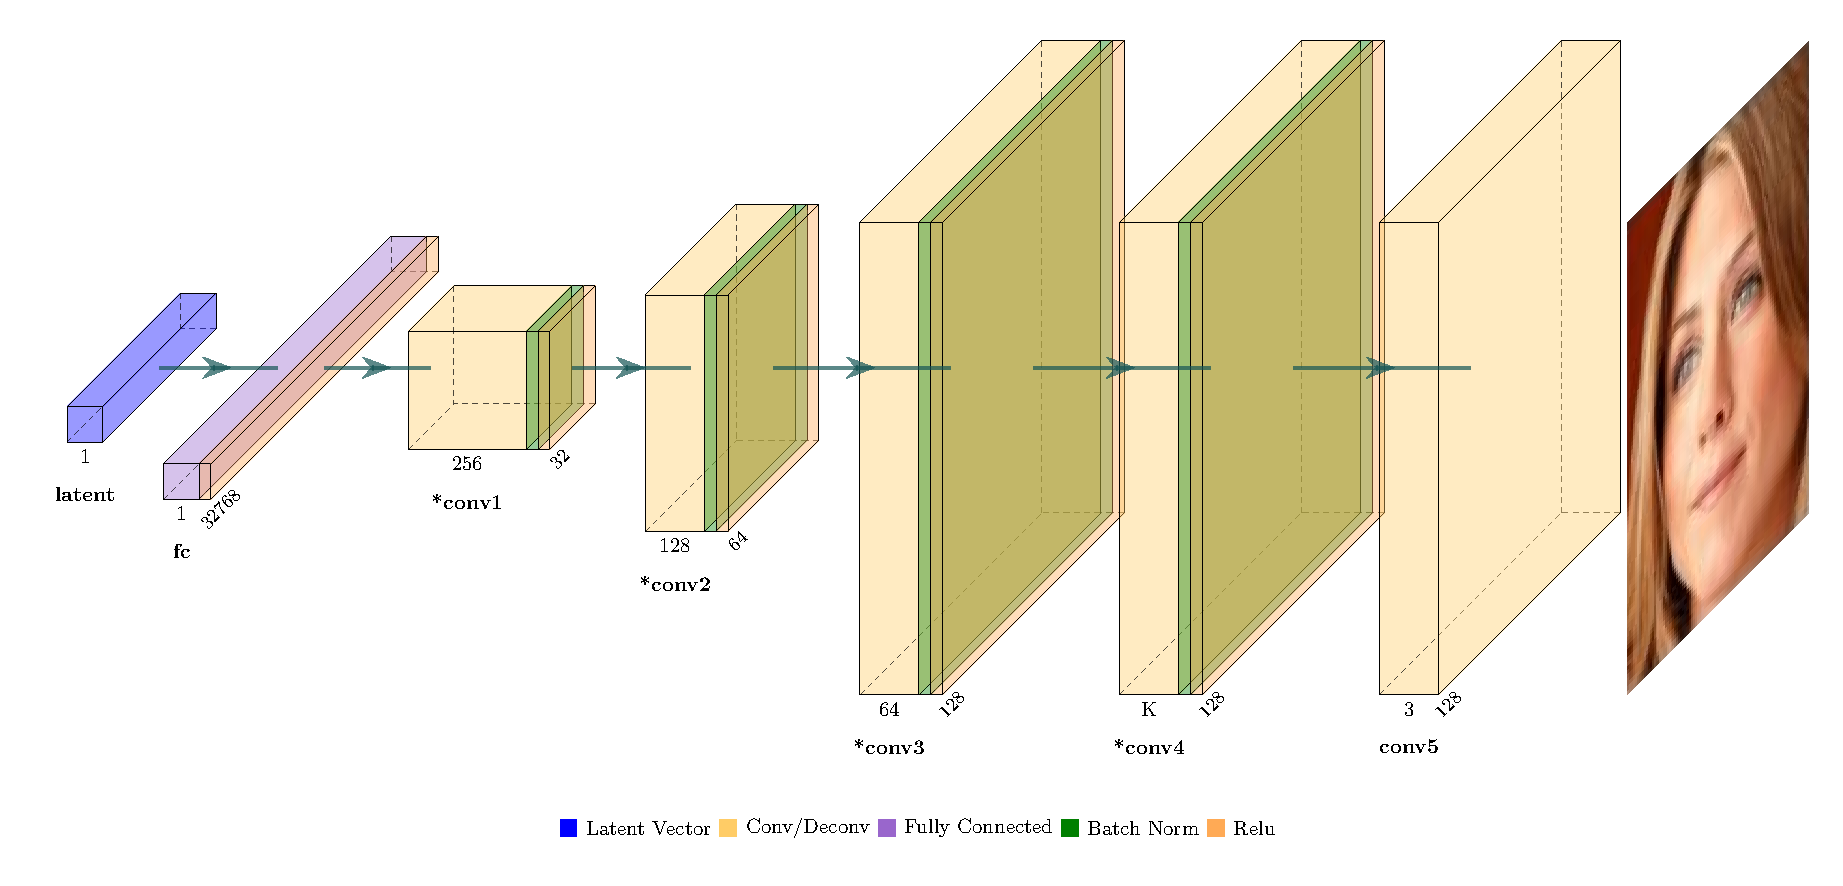
\includegraphics[width=0.9\textwidth]{cnn.pdf}
	\end{figure}}
		\end{itemize}
	\end{itemize}
\end{frame}

 
\end{document}